\documentclass{article}[18pt]
\usepackage{../../../format}
\lhead{Software Engineering - Software Development}


\begin{document}
\begin{center}
\underline{\huge SDLC and Standards}
\end{center}
\section{Software Development Lifecycle}
\begin{center}
	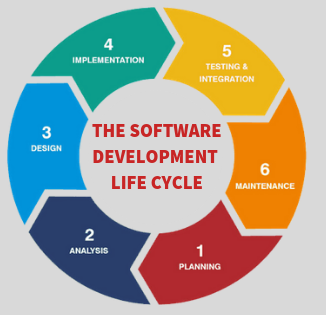
\includegraphics[scale=0.7]{Lifecycle}
\end{center}
\begin{itemize}
	\item The SDLC framework is used in industry to design, develop and test high quality software
	\item Focussing on creating software that meets the needs and expectations of the client
	\item Within the client's timeline and budget
\end{itemize}
\section{Phases}
\subsection{Planning and RE(requirements) analysis}
\begin{itemize}
	\item Planning is the first and most fundamental of the phases
	\item Get this wrong and nothing else will work
	\item Inc. quality assurance and risk analysis
\end{itemize}
Stakeholders/Roles within this phase
\begin{itemize}
	\item Client
	\item Customer
	\item Approver (managerial oversight)
	\item Assessor (some degree of technical expertise to advise)
\end{itemize}
Outcome
\begin{itemize}
	\item An approved proposal
	\item A functional requirements doc
\end{itemize}
\subsection{Design}
\begin{itemize}
	\item The goal here is to create the s/w design document(s) based on the inputs from the previous phase (planning and analysis)
	\item Perform design discussions, examine design patterns, consider requirements
	\item Output: systems design docs for DB, API, application, infrastructure, testing, training, maintenance, user ...
\end{itemize}
Roles:
\begin{itemize}
	\item \textbf{End user} - final users of system
	\item \textbf{Business analyst} - provide requirements to the design team, review solution design and artefacts
	\item \textbf{Project Manager} - Finalize data conversion strategy and test strategy, review solution design and artefacts
	\item \textbf{Technical-Architect, Tech-Designer, Design-Team} - Design system architecture, software components, etc; design walk-through
	\item \textbf{Developer/Construction Team} - Assist with identifying and finalizing testing strategy; review of the architecture and software components
	\item \textbf{Database team} - Assist with architecture design and data conversion strategy
\end{itemize}
\subsection{Implementation}
\begin{itemize}
	\item Get your hands dirty with coding
	\item Your teams may use any approach that works for you
	\item Within a business you will have to abide by their coding guidelines
\end{itemize}
Roles:
\begin{itemize}
	\item \textbf{Customer}, sponsor and signs off team effort; review progress with the developers and the PM.
	\item \textbf{Project Manager}, resolve resource, scheduling, budget issues; review and report progress.
	\item \textbf{Developer}, construct a working solution from the approved design; produce artifacts and put them under configuration control and perform change control; employ tools, systems and conform to prescribed standards (platforms, coding practices, programming languages, etc) that are in line with the organization’s objectives.
	\item \textbf{Database Administration Group}, assist with implementing the solution design and data conversion strategy.
	\item \textbf{Implementation supervisor/manager}, assist with identifying the requirements for implementation of the solution (which includes system readiness, resources, time-lines).
	\item \textbf{Integration supervisor/manager}, identify how integration of the solution in a new hardware/software  environment would be achieved; what tests are required to evaluate integration.
\end{itemize}
\subsection{Testing \& Integration/Deployment}
\begin{itemize}
	\item These phases are sometimes separated
	\item The goal of testing is to check that the development is functional and meets requirements
	\item Complexity arises from integration of a novel system with existing (sub-)systems
	\item Test for various functional attributes
	\begin{itemize}
		\item Security, conformance, accessibility, performance, stress
	\end{itemize}
\end{itemize}
Roles:
\begin{itemize}
	\item \textbf{Project Manager}, resolve resource, scheduling, budget issues; review and report progress.
	\item \textbf{Developer}, assist with building tests and analysis of test results.
	\item \textbf{Database Administration Group}, assist with integration of the solution design and data conversion tests.
	\item \textbf{Implementation manager}, assist with analysis of test results.
	\item \textbf{Integration manager}, assist with analysis of test results.
\end{itemize}
Sign off is completed when the functional requirements specification has been met
\subsection{Implementation}
\begin{itemize}
	\item Some versions of the SDLC have an additional phase here
	\item The focus is to install the system in the production environment and to bring it into \textbf{operation}; and then to ensure that the system:
	\begin{itemize}
		\item Satisfies the functional requirements
		\item Satisfies the business needs
		\item Adheres to all mandates, physical constraints and service level agreements
		\item Operates as described in the User and Operator Manuals
	\end{itemize}
\end{itemize}
\subsection{Maintenance}
\begin{itemize}
	\item On successful operational transfer of the project, development group hands over to the maintenance group
	\item Documentation must be ready for transfer at this time
	\item Roles:
	\begin{itemize}
		\item \textbf{Solution Delivery Team} – Prepares all solution documentation 
		and manuals for the maintenance group.  The solution delivery 
		team will supply any requested training to help maintenance 
		team technicians learn the solution’s behaviours
		\item \textbf{Solution Maintenance Team} – Reviews all solution 
		documentation and supports the solution until the terms 
		of the maintenance agreement expire
	\end{itemize}
\end{itemize}
\section{Alternatives}
There are many correct models depending on the people and project. The SDLC just outlines the phases
\section{Standards}
Why standards?
\begin{itemize}
	\item Quality
	\item Shared communication
	\item Shared understanding
	\item Influence, from understanding to creation/development
	\item Profit
	\item Collaboration
	\item Reputation
	\item Regulation (assurance)
	\item Flexibility
\end{itemize}
Importance
\begin{itemize}
	\item They encapsulate best practice (normally)
	\item Framework for QA
	\item Provide continuity
	\begin{itemize}
		\item Record of decision making process
		\item Organisational memory
		\item New staff save time
	\end{itemize}
\end{itemize}
Issues:
\begin{itemize}
	\item Standards are considered too large, unwieldy and difficult to adopt for SMEs
	\item Focus is on large organisations
	\item Concerns over cost and documentation
	\item Difficult to justify
\end{itemize}
\section{ISO SC7}
\subsection{Structure}
\begin{center}
	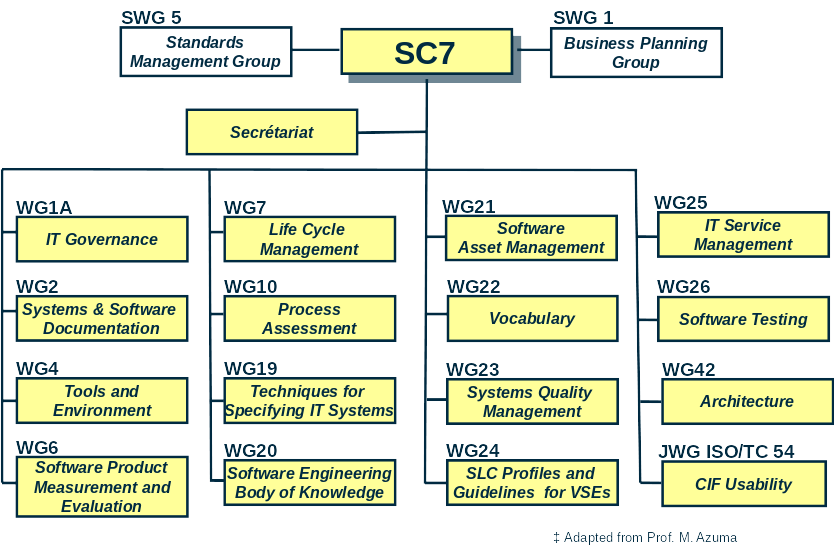
\includegraphics[scale=0.7]{SC7}
\end{center}
\subsection{Domains}
\begin{center}
	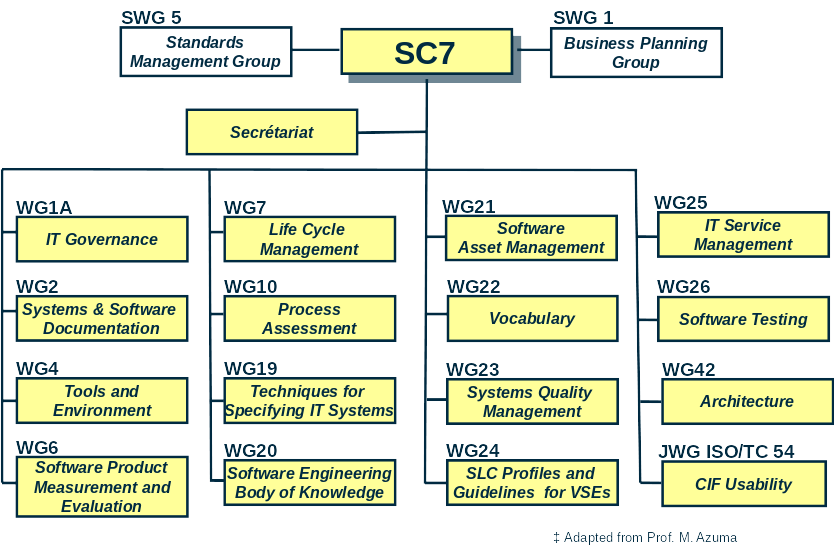
\includegraphics[scale=0.7]{Domains}
\end{center}
\subsection{Standards}
\begin{center}
	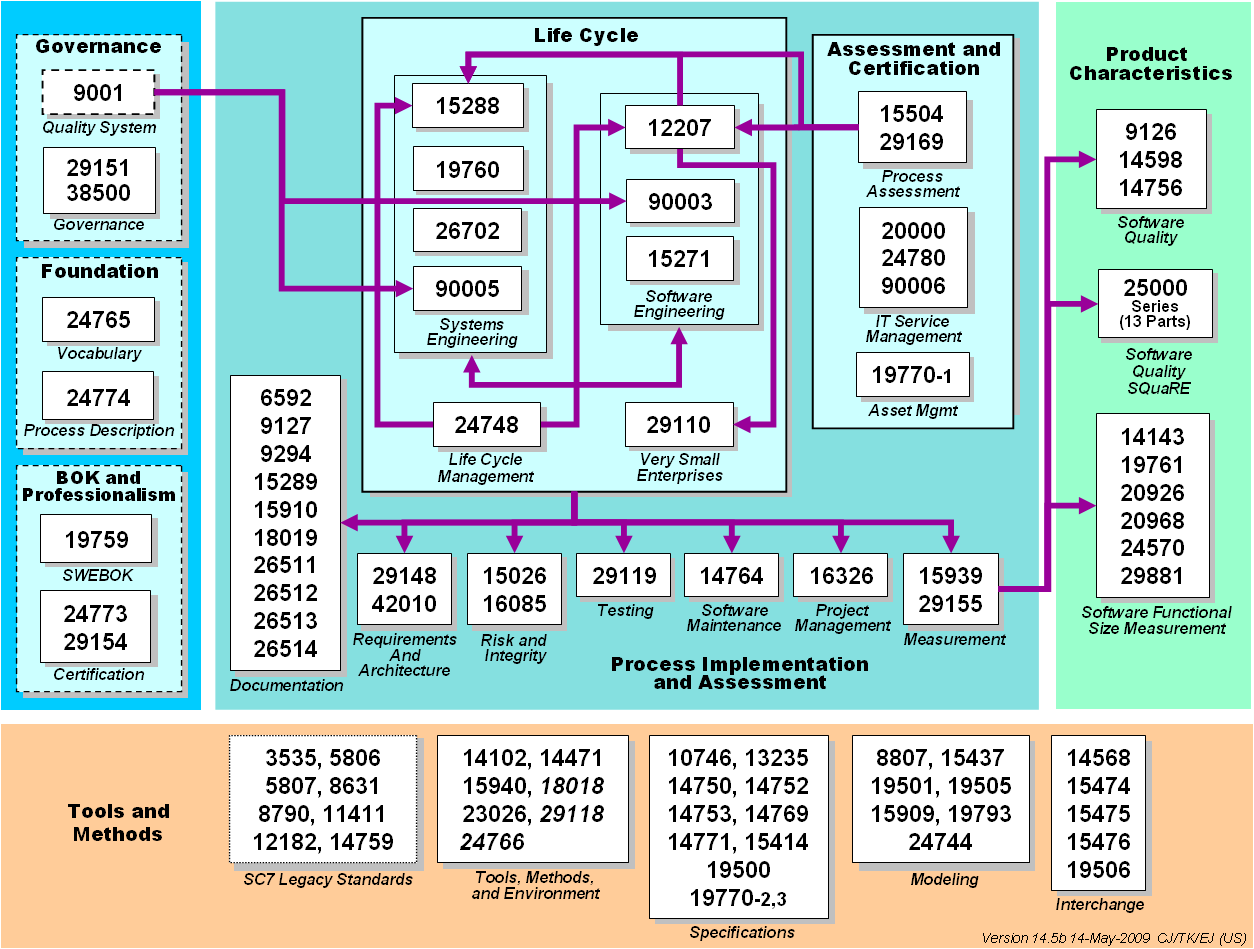
\includegraphics[scale=0.7]{Standards}
\end{center}
Standards of particular interest
\begin{itemize}
	\item ISO 9000, family of standards for quality management systems
	\item ISO 12207, defines the software engineering process, activity, and tasks that are associated with a software life cycle process from conception through retirement
	\item ISO 15504, also known as SPICE (Software Process Improvement and Capability Determination), is a framework for the assessment of processes
\end{itemize}
\section{ISO 9000}
\begin{center}
	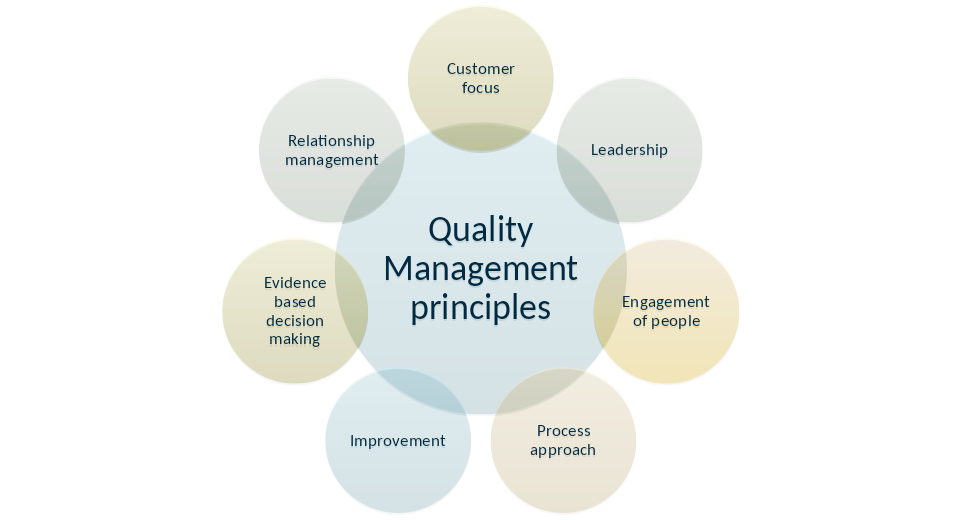
\includegraphics[scale=0.7]{ISO9000}
\end{center}
QSM:
\begin{itemize}
	\item ISO9001 – QSM for Quality Assurance in design, development, production, installation and service
	\item ISO9002 – QSM for Quality Assurance in production, installation, and servicing
	\item ISO9003 – QSM for Quality Assurance in final inspection and test
\end{itemize}
Quality: refers to all features of a product (such as software) which are required by a customer\\
\\
Quality management: covers the organisations approach to ensuring that it produces quality products and complies with the appropriate regulations
\section{ISO 12207}
\begin{itemize}
	\item Created to supply a common structure so that the buyers, suppliers, developers, maintainers, operators, managers and technicians involved with the software development use a common language
	\item It is the standard that defines all the tasks required for developing and maintaining software
	\item Created in ’95, last updated in ’17 (ISO 12207:2017)
	\item Covers the process in the life cycle of software:
	\begin{itemize}
		\item High level process architecture
		\item Activities and tasks
		\item Tailored for any organization or project (inc. SME et al)
		\item An ‘inventory’ of processes from which to choose
	\end{itemize}
	\item This standard does not create a standardised way to create a product
	\item It is not prescriptive
	\item Nor does it advocate or enforce a standardised methodology
\end{itemize}
\subsection{ISO 12207:17}
\begin{center}
	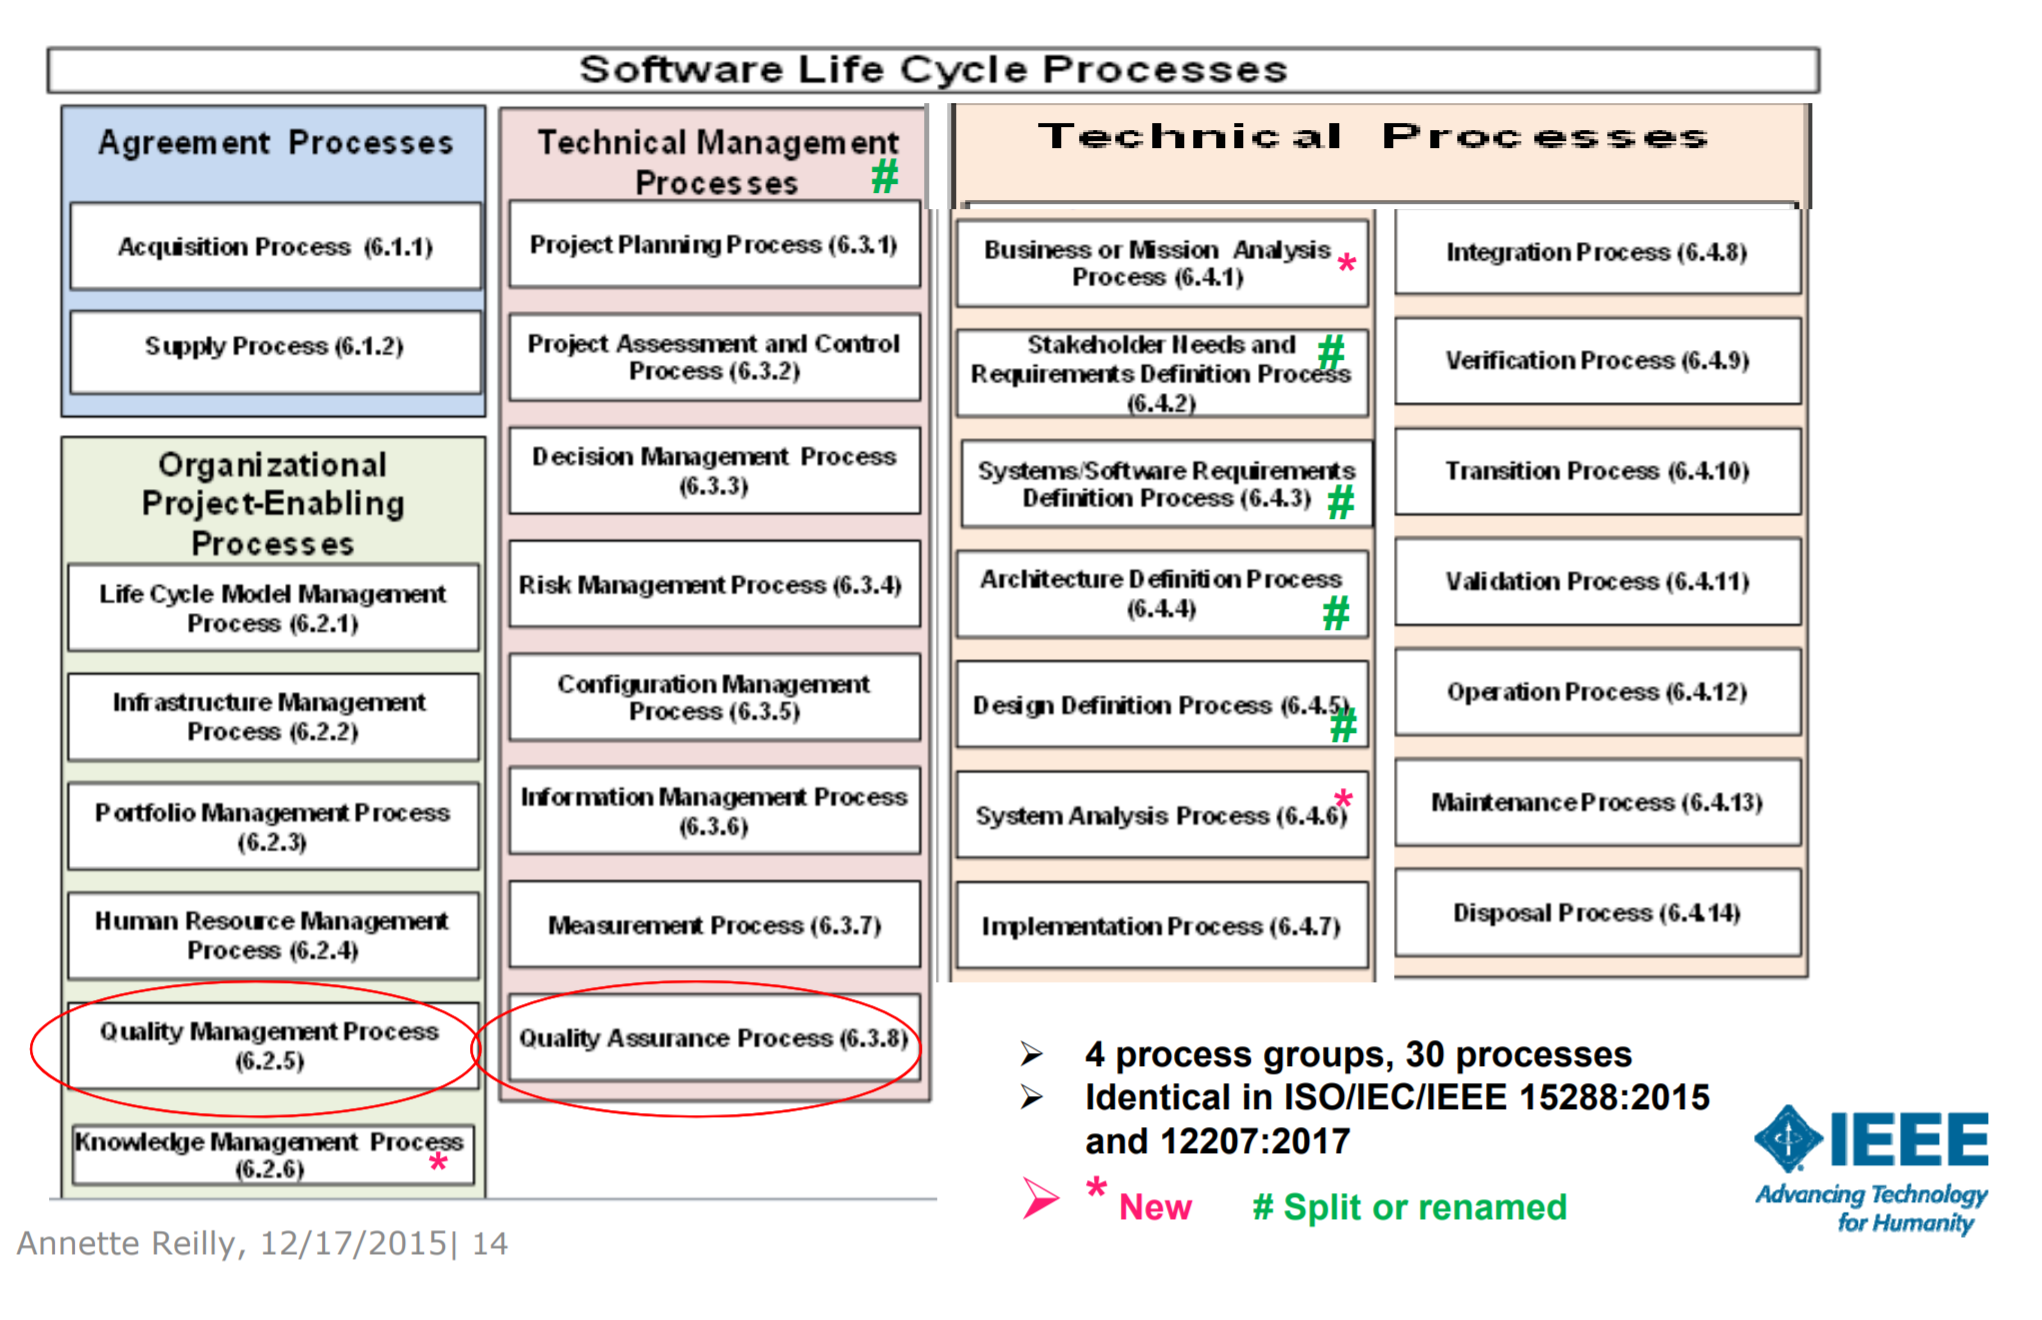
\includegraphics[scale=0.7]{ISO12207:17}
\end{center}
\section{Process Implementation}
\begin{itemize}
	\item Define or select software life cycle model appropriate to the scope, magnitude, and complexity of the project;
	\item Select, tailor, and use standards, methods, tools, and programming languages (if not stipulated in  contract);
	\item Develop plans for conducting the activities of the Development process.
\end{itemize}
\section{ISO 15504}
Process assessment: What is it?
\begin{itemize}
	\item A disciplined examination of the processes by an organisation against a set of criteria to determine capability of those processes to perform within quality, cost and schedule goals
	\item Focus here is on continual, self-improvement
\end{itemize}
Why bother?
\begin{itemize}
	\item Identify strengths and weaknesses in current utilisation of processes
	\item Ongoing development of systems, maturity and growth
	\item Feeds into the future
\end{itemize}
\begin{center}
	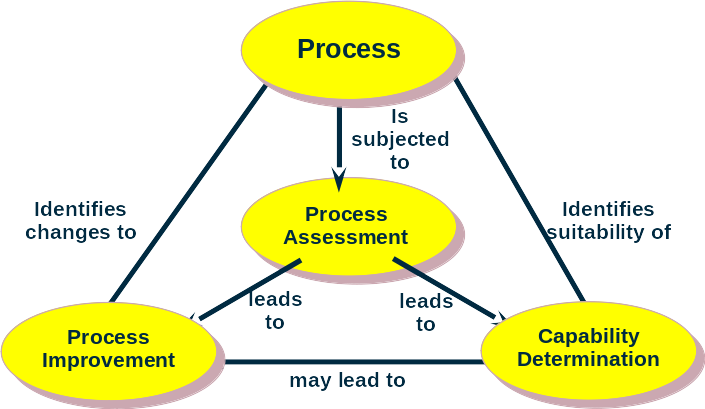
\includegraphics[scale=0.7]{ISO15504}
\end{center}

\end{document}